\documentclass[11pt, oneside]{article}
\usepackage{geometry}
\usepackage{graphicx}
\usepackage{amssymb}
\usepackage{amsmath}
% \usepackage{apacite}
\usepackage{fancyhdr}
\usepackage{lastpage}
\usepackage{graphicx, wrapfig, subcaption, setspace, booktabs}
\usepackage[T1]{fontenc}
\usepackage[font=small, labelfont=bf]{caption}
\usepackage{fourier}
\usepackage[protrusion=true, expansion=true]{microtype}
\usepackage[english]{babel}
\usepackage{sectsty}
\usepackage{url, lipsum}
\usepackage{mathtools}
\usepackage{listings}
\DeclarePairedDelimiter{\floor}{\lfloor}{\rfloor}

\geometry{letterpaper}

\newcommand{\HRule}[1]{\rule{\linewidth}{#1}}
\onehalfspacing
\setcounter{tocdepth}{5}
\setcounter{secnumdepth}{5}

%-------------------------------------------------------------------------------
% HEADER & FOOTER
%-------------------------------------------------------------------------------
\pagestyle{fancy}
\fancyhf{}
\setlength\headheight{15pt}
\fancyhead[L]{Student ID: 3032162875}
\fancyhead[R]{University of California, Berkeley}
\fancyfoot[R]{Page \thepage\ of \pageref{LastPage}}

%-------------------------------------------------------------------------------
% TITLE PAGE
%-------------------------------------------------------------------------------
\title{
  \normalsize \textsc{Chapter 1} \\ [2.0cm]
  \HRule{0.5pt} \\
  \LARGE \textbf{\uppercase{
  Time Series Forecasting of Monthly Active Users with Long Short-Term Memory
      Networks
  }}
  \HRule{2pt} \\ [0.5cm]
  \vspace*{5\baselineskip}
}
\author{
  Matthew Louis Rosendin \\
  University of California, Berkeley \\
  Department of Industrial Engineering and Operations Research
}
\date{April 13, 2018}

%-------------------------------------------------------------------------------
% DOCUMENT
%-------------------------------------------------------------------------------

\begin{document}
\maketitle
\newpage

\tableofcontents
\newpage

\listoffigures
\newpage

\section{Introduction}
Our project, in partnership with Adobe Systems Inc., is an interactive dashboard that forecasts monthly active users for any Adobe software product. We've accomplished forecasts with excellent accuracy as far as 5 months into the future. The growth model's forecast can be used for a number of reasons, including as an input to forecasting revenue or as a measure of product health. While forecasting monthly active users is nothing new, our application of artificial neural networks (ANNs) seems to be a novel approach that has yielded promising results.

In this chapter of the paper I analyze and discuss the implications of our model's performance and describe my work in deploying our model. I begin by explaining the concrete goals of this work, then outlining the motivation, before finally diving into a technical introduction to our model. Following the basic conceptual discussion around our model, I start the discussion about how I refined the "raw" model code into a flexible, scalable, and configurable object. The translation of the model into a manageable machine learning software system led to additional improvements to the model, such as hyperparameter optimization. A byproduct of the optimization was an exhaustive experimentation of model performance metrics. The underpinning of the preceding work is the user interface. I discuss my work in front-end and systems engineering that resulted in the final deliverable: a forecasting dashboard powered by machine learning.

\subsection{Goal}
Our team's foremost goal is to create a practical and interactive product growth model for Adobe senior management. My individual goal was to design and create a user interface to interact with the model. Throughout my contributions, I've added additional value around testing the performance of our model and gathering relevant metrics.

\subsection{Motivation}
The motivation for creating a dashboard is straightforward. The dashboard enables the user to train the machine learning model resulting in performance metrics and the monthly active user forecast.
The motivation for the section on hyperparameter optimization was simply to improve the results of our model. From the resulting tests, we've found that our model's forecasting capability had improved. Part of the discussion in this paper is reserved for analyzing the source of model improvement.

\subsection{Time Series Forecasting}

In order to explain why we chose our particular model (a long short-term memory network) I will explain the characteristics of the problem we are solving through a brief taxonomy. The problem is best framed as, "how do we forecast monthly active usage multiple weeks into the future?". The most salient characteristic of this problem is that the data is a long sequence (i.e., data is chronologically ordered) of values, known as a time series. What we are trying to achieve is a forecast of time series data, so the solution to the problem is known as time series forecasting.

\subsection{Autoregressive Models}

The simplest model might be an autoregressive (AR) model in which the forecast values are regressed on prior data:

\begin{equation}
  \label{eq:1}
  X_t = c + \sum_{i=1}^p \phi_i X_{t-i} + \epsilon_t
\end{equation}

where $c$ is a constant, $\epsilon_t$ is an error term, and $\phi_1, ..., \phi_p$ are the parameters to be estimated by linear regression. To forecast a value for the present time $t$, we specify a parameter $p$, known as the "order" or "lag". With $p=3$ the corresponding model would look like this:

\begin{equation}
  \label{eq:2}
  X_t = c + \phi_1 X_{t-1} + \phi_2 X_{t-2} + \phi_3 X_{t-3} + \epsilon_t
\end{equation}

We would call this an autoregressive model with a lag of 3 time steps where time steps are defined as the number of sequential data points. The autoregressive model can be notated as $AR(3)$ to indicate its order with $p=3$.

In our work we use the concept of "lag" from the autoregressive model in our supervised learning model. Our dataset is multivariate, meaning there are more than two observations for each time step. Since we would like to forecast multiple weeks into the future, our model is multi-stepped.

\subsection{Recurrent Neural Networks}

There are many good reasons to justify using an artificial neural network. Much of the recent literature on time series forecasting is focusing on the advantage of ANNs versus other methods, including autoregressive interactive moving average (ARIMA) models. For instance, Ahmed et al. and Zhang show that ANNs are shown to be superior for generalized time series problems \cite{ahmed et al.}. Although complex models such as neural networks can hard to interpret, our project team values performance over interpretability. Furthermore, we have designed features similar to those in financial time series models. For financial stock data, Adebiye et al. show that ANNs are superior to ARIMA models \cite{adebiye et al.}. Lastly, ANNs are capable of modeling non-linearities which can improve the forecast.

\begin{figure}[h]
  \caption{Diagram of a one-unit Long Short-Term Memory (LSTM) network \cite{deloche}}
  \centering
  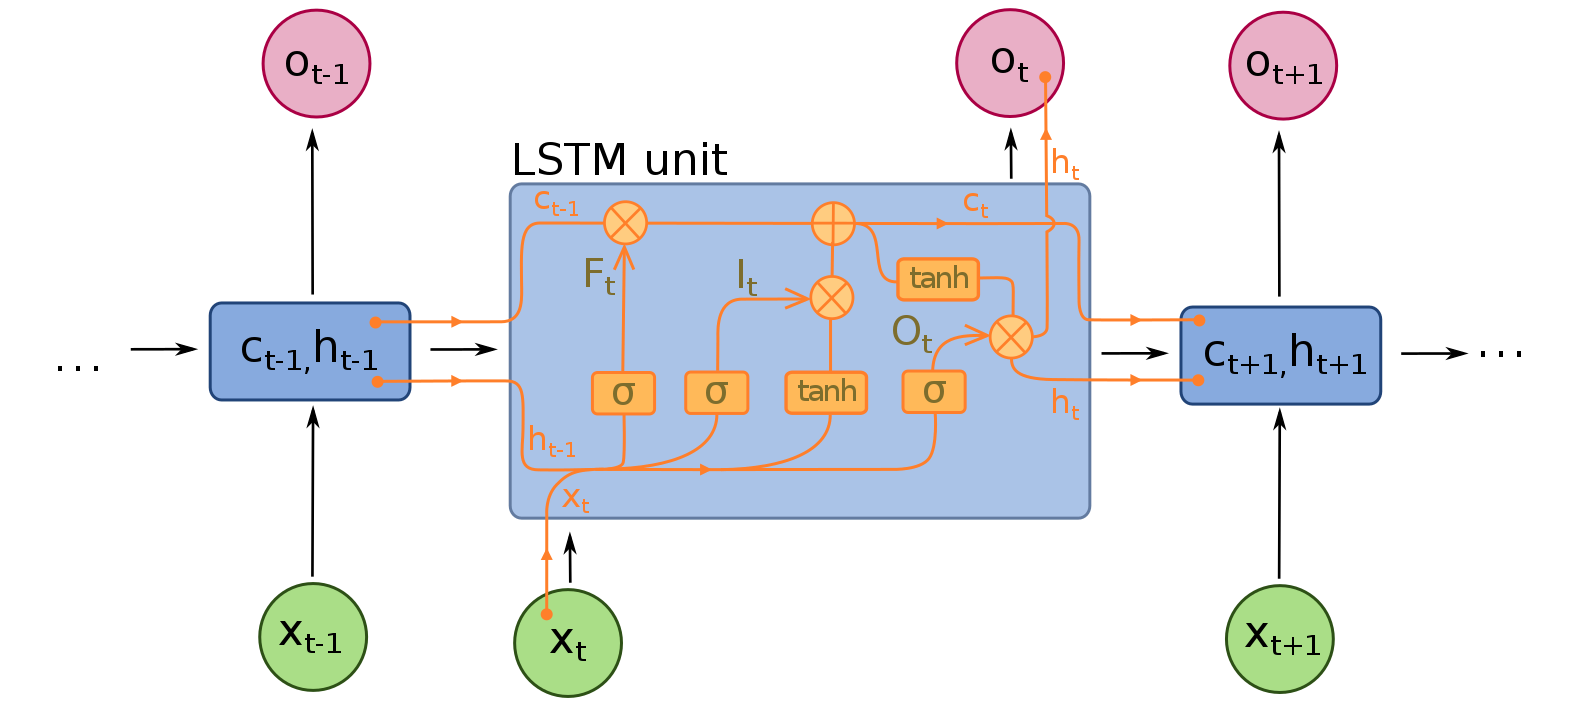
\includegraphics[width=12.5cm]{images/Long_Short-Term_Memory.png}
\end{figure}

Recurrent neural networks (RNNs) are a class of artificial neural network where connections between units form a directed graph along a sequence. In other words, RNNs retain state at one time to the next, using the previous state's output for the current estimate. This characteristic enables multi-stepped time series forecasting. A particular architecture of RNNs known as Long Short-Term Memory (LSTM) allows the model to recognize and retain short-term patterns for long periods of time. This architecture is used best where data from an earlier state needs to be recalled at a later state. Examples of LSTM networks in industry include Google Voice \cite{beaufays}.

\section{Object-Oriented Abstraction}
The working LSTM model was created in a Jupyter Notebook. While serving as a minimum proof of concept, the model should not require the end-user engage directly with code. Furthermore, the following criteria were set: 1) the lifecycle of the model (from training, testing, to final predictions) needed to be automated and callable with one command; 2) the Jupyter Notebook code (which executes similarly to a script) needed to be organized into an object-oriented structure to store data within the object instance; 3) the model needed to be capable of loading datasets of arbitrary products. Criterion (2) is more a matter of preference and style to the author, as other programming paradigms could be considered. The rest of this section briefly discusses the process involved in restructuring the model code to meet the criteria.

\subsection{Decomposition}
The goal of decomposition is to break a complex system into parts that are easier to understand, program, and maintain. The process of decomposing the Jupyter Notebook code involved defining separate modules for loading datasets (\texttt{data.py}), feature engineering (\texttt{features.py}), training/testing/predicting (\texttt{core.py}), and accessing utilities (\texttt{utils.py}). Furthermore, the code was organized into functions, and eventually into methods (discussed below).

\subsection{Encapsulation}
After breaking the code into manageable chunks, I created a Python class wrapper to store internal state and to allow the end-user to specify runtime options. The entire model can be run by using the wrapper's simple application programming interface (API).

\section{Hyperparameter Optimization}
Hyperparameter optimization deals with the learning parameters of a model rather than weights for features. While I made a significant effort in this area, the optimization was only run on one machine. Increasing compute resources to perform a more extensive search may yield further interesting results.

\subsection{Cross-validation}
\label{cross_validation}
In time series problems, cross-validation is performed chronologically with splits at fixed time intervals. In my trials, I ran cross-validation with 2, 3, and 10 splits. I wanted to understand the change in our key metric, MAPE (mean absolute percent error), as the number of splits $S$ increases. According to the \texttt{scikit-learn} documenation, the training set $Tr$ for the $i$th split has a size

\begin{equation}
  \label{eq:3}
  Tr_{i} = \floor*{\frac{i \times N}{(S + 1)}} + N \bmod (S + 1)
\end{equation}

where $N$ is the number of samples, $S$ is the number of splits, and $\floor{expression}$ denotes the floor function. Meanwhile, the test set $Te$ has the following size:

\begin{equation}
  \label{eq:4}
  Te_{i} = \floor*{\frac{N}{(S + 1)}}
\end{equation}

For time series splits with $S>1$, the sum of the first train/test set is strictly less than $N$ and the last train/test set is equal to $N$:

\begin{equation}
  \label{eq:5}
  Tr_{i} + Te_{i} < N \quad \forall i \in \{1, \dots, S-1\}
\end{equation}

\begin{equation}
  \label{eq:6}
  Tr_{S} + Te_{S} = N
\end{equation}

These equations describe the train/test split pairs. It is important to note that the chronological indexing of the data is preserved for both input data and additional "held-out" data. This splitting strategy helps validate the results of the exhaustive hyperparameter search that is described in the next section.
\subsection{Grid Search}
This search algorithm is simple. It exhaustively generates candidate learning parameters and selects the best candidate based on the scoring function (MAPE). Each candidate undergoes the time series splitting strategy discussed in Section \ref{cross_validation} to help validate the candidate's score. Further discussion about alternative algorithms is in Section \ref{improving_hyperparameter_optimization_efficiency}.

\subsection{Results}
An example of the output this process is shown in Figure~\ref{fig:Example_Output}.

\begin{figure}[h]
  \caption{Example output: 5.79\% MAPE}
  \label{fig:Example_Output}
  \begin{center}
    \begin{tabular}{c}
      \begin{lstlisting}
        Parameters: {
          'batch_size': 150,
          'epochs': 200,
          'optimizer': 'adam',
          'units': 100
        }
        Test loss: [128.97596047141334, 128.97596047141334]
        Testing set RMSE: 24318.87
        Testing set MAPE: 5.79%
        Testing set sMAPE: 0.06%
      \end{lstlisting}
    \end{tabular}
  \end{center}
\end{figure}

\section{Systems Engineering}
I worked to productionize our model by building a back-end that is capable of extracting and preparing data, training and validating the model, and producing forecasts. The back-end performs the business logic computation without end-user interaction. The back-end was written entirely in Python and its component parts are discussed in this section.

\subsection{Server Infrastructure}
All software written for this project was developed and tested on local machines. System specifications of the host machine producing the results in this report are shown in Figure~\ref{fig:System_Specs}. The system runs Python 3.6.4 and we've tested on local machines (macOS) and a Docker virtual host container running Ubuntu 16.04 (see Section \ref{distributed_machine_learning_clusters} for further discussion about Docker). A simple web server framework, Flask (\url{http://flask.pocoo.org/}), is employed to interact with the front-end (see in Section \ref{user_interface}). A basic API has been developed to enable asynchronous communication with the front-end client device.

\begin{figure}[h]
  \caption{Host machine system information}
  \centering
  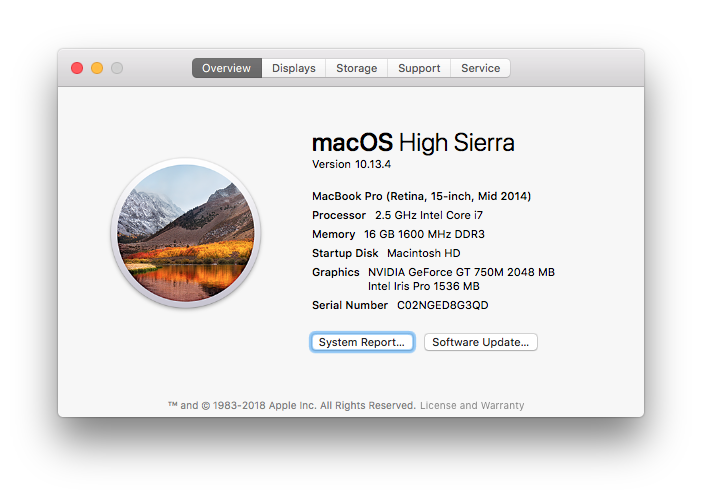
\includegraphics[width=12.5cm]{images/System_Specs.png}
  \label{fig:System_Specs}
\end{figure}

\subsection{Distributed Task Queue}
Since the machine learning processes are long-running processes, an open-source distributed task queue called Celery (\url{http://www.celeryproject.org/}) is used to manage the scheduling, status, and output. When the user uses the front-end to make a new forecast, an API endpoint queues the task. In our case, there was only one client utilizing the queue at a time. However, the additional benefit of using a task queue is to coordinate background jobs. When the end-user begins a new forecast task, they receive a response from the server immediately. The code on the client polls another API endpoint every second to check the status of the forecast task. When the status appears successful, the server responds with the necessary data to render the visualizations on the client device, as well as summary statistics.

\section{User Interface}
\label{user_interface}
\subsection{Forecast Visualization}
\begin{figure}[h]
  \caption{Dashboard user interface}
  \centering
  \fbox{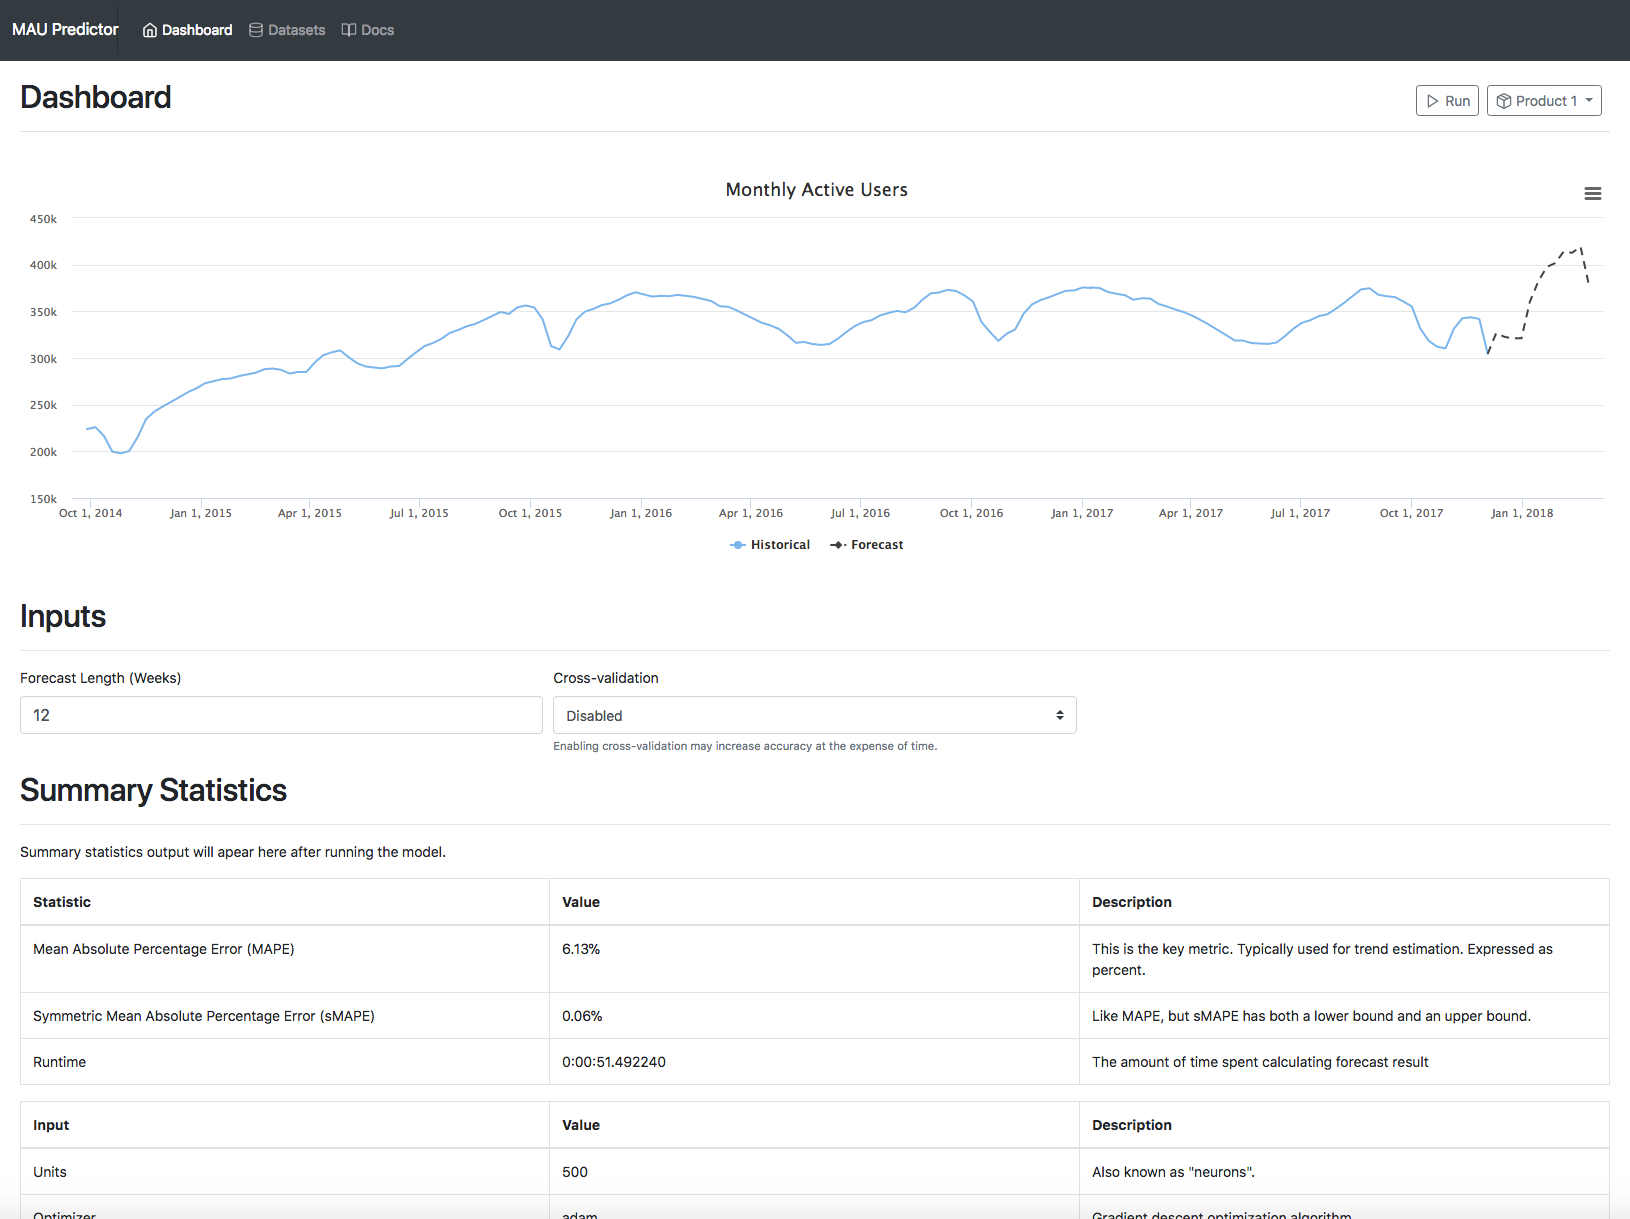
\includegraphics[width=12.5cm]{images/Dashboard.png}}
\end{figure}

\begin{figure}[h]
  \caption{Product 1 trend: 6.24\% MAPE}
  \centering
  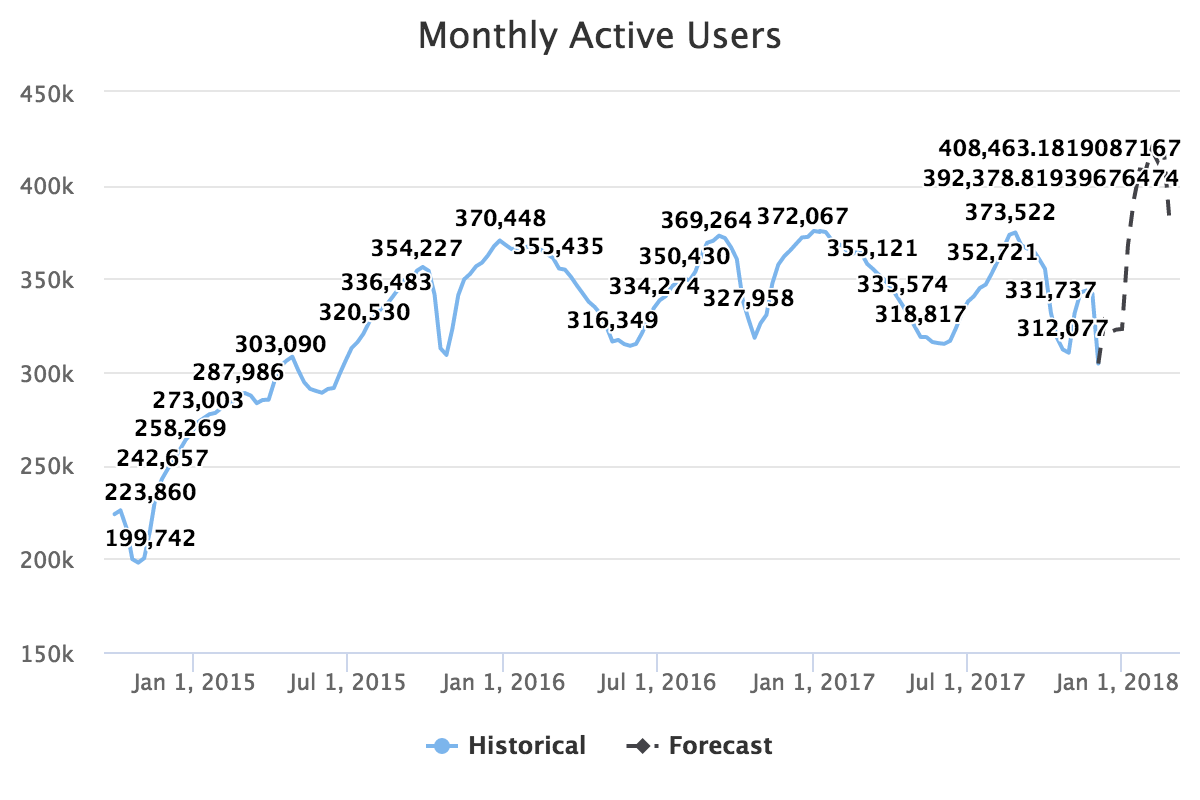
\includegraphics[width=12.5cm]{images/Product_1-Trend-6_24_Percent_MAPE.png}
  \label{fig:Product_1-Trend}
\end{figure}

Figure~\ref{fig:Product_1-Trend} shows the historical monthly active user trend of Product 1 with the 12 week forecast in the dashed line.

\begin{figure}[h]
  \caption{Product 1 forecast: 6.24\% MAPE}
  \centering
  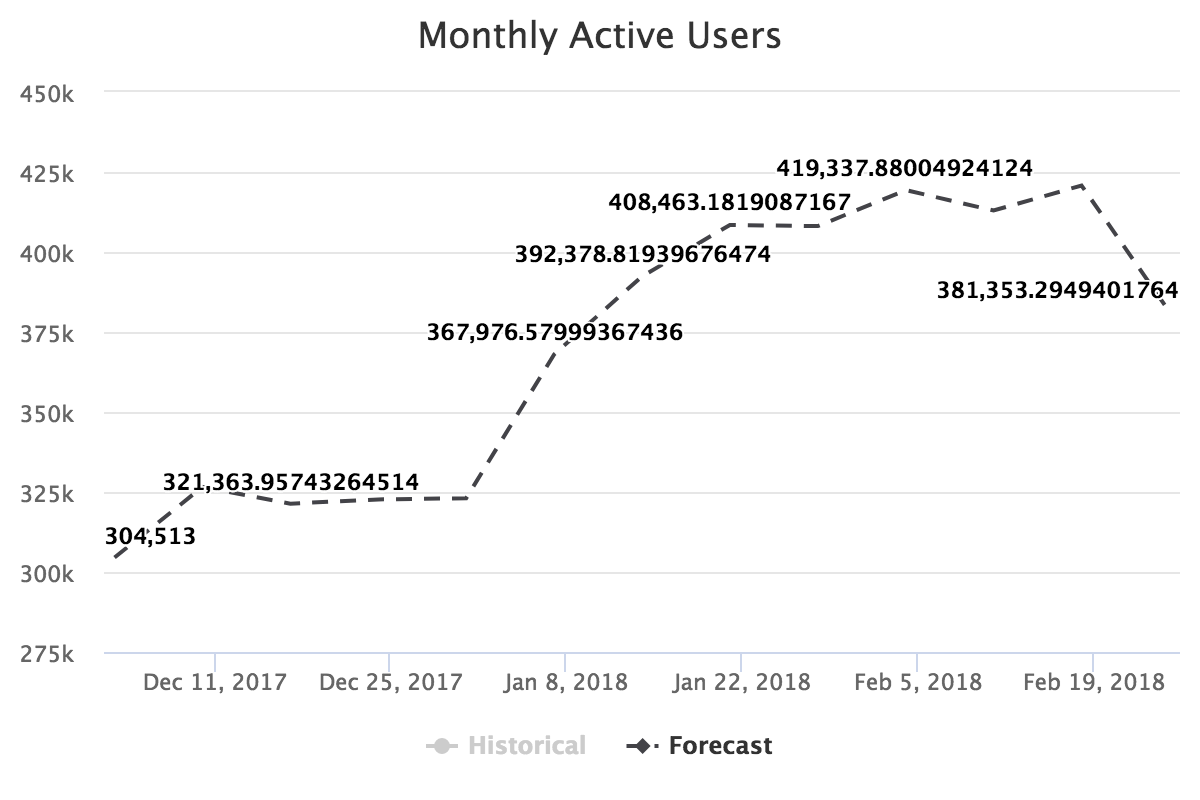
\includegraphics[width=12.5cm]{images/Product_1-Forecast-6_24_Percent_MAPE.png}
  \label{fig:Product_1-Forecast}
\end{figure}

Figure~\ref{fig:Product_1-Forecast} shows the forecast for Product 1 over a 12 week period (December 3rd - February 25th 2018).

\subsection{Documentation}
Wrote documentation (akin to a usage guide)

\section{Next Steps}
\subsection{Websockets}
Improve job monitoring; rather than polling every second with HTTP calls, open a websocket channel.
\subsection{Data Pipeline Automation (Apache Hadoop)}
\subsection{Dimensionality Reduction by Feature Selection}
\subsection{Improving Hyperparameter Optimization Efficiency}
  \label{improving_hyperparameter_optimization_efficiency}
  The brute-force search algorithm used to optimize hyperparameters can probably be replaced with another. The \texttt{GridSearchCV} class from \texttt{scikit-learn} implements the algorithm that was used for our project, but other hyperparameter optimizers are available in the \texttt{model\_selection} module of \texttt{scikit-learn}. The other options include a randomized search where a subset of the parameter grid is sampled. This requires passing in distributions of the hyperparameters themselves, which could be an interesting opportunity to avoid an exhaustive search.

\subsection{Confidence Interval Visualization}
A major upgrade would be a visualization of forecast confidence intervals on the current graph.

\subsection{Distributed Machine Learning Clusters}
\label{distributed_machine_learning_clusters}
Docker containers can be scaled on nodes in a distributed system.

\section{Conclusion}
In conclusion, ...

\begin{thebibliography}{9}
  % Time series forecasting using a hybrid ARIMA and neural network model
  % https://www.sciencedirect.com/science/article/pii/S0925231201007020

  % Comparison of ARIMA and Artificial Neural Networks Models for Stock Price Prediction
  % https://www.hindawi.com/journals/jam/2014/614342/

  % Hyperparameter optimization - Wikipedia
  % https://en.wikipedia.org/wiki/Hyperparameter_optimization

  % Bayesian information criterion - Wikipedia
  % https://en.wikipedia.org/wiki/Bayesian_information_criterion

  % Building Intelligent Systems: A Guide to Machine Learning Engineering
  % https://books.google.com/books?id=s91PDwAAQBAJ

  % Scaling up Machine Learning
  % https://books.google.com/books?id=9u0gAwAAQBAJ

  % Hidden Technical Debt in Machine Learning Systems
  % https://papers.nips.cc/paper/5656-hidden-technical-debt-in-machine-learning-systems.pdf

  % Diagram of a one-unit Long Short-Term Memory (LSTM) network
  % https://commons.wikimedia.org/w/index.php?curid=60149410

  \bibitem{adebiye et al.}
  Adebiyi, A. A., Adewumi, A. O., \& Ayo, C. K. (2014). Comparison of ARIMA and Artificial Neural Network Models for Stock Price Prediction. \textit{Journal of Applied Mathematics}, \textit{2014}.

  \bibitem{ahmed et al.}
  Ahmed, N. K., Atiya, A. F., Gayar, N. E., \& El-Shishiny, H. (2010). An Empirical Comparison of Machine Learning Models for Time Series Forecasting. \textit{Econometric Reviews}, \textit{29}(5-6).

  \bibitem{beaufays}
  Beaufays. (2015, August 11). The neural networks behind Google Voice transcription [Blog post]. Retrieved from https://research.googleblog.com/2015/08/the-neural-networks-behind-google-voice.html.

  \bibitem{deloche}
  Deloche, Fran\c{c}ois. (2017). Diagram of a one-unit Long Short-Term Memory (LSTM) network. Retrieved from https://commons.wikimedia.org/w/index.php?curid=60149410.

  % Google voice search: faster and more accurate
  % https://research.googleblog.com/2015/09/google-voice-search-faster-and-more.html
\end{thebibliography}

\end{document}
